
\documentclass[paper-main.tex]{subfiles}
\begin{document}


\begin{figure*}
    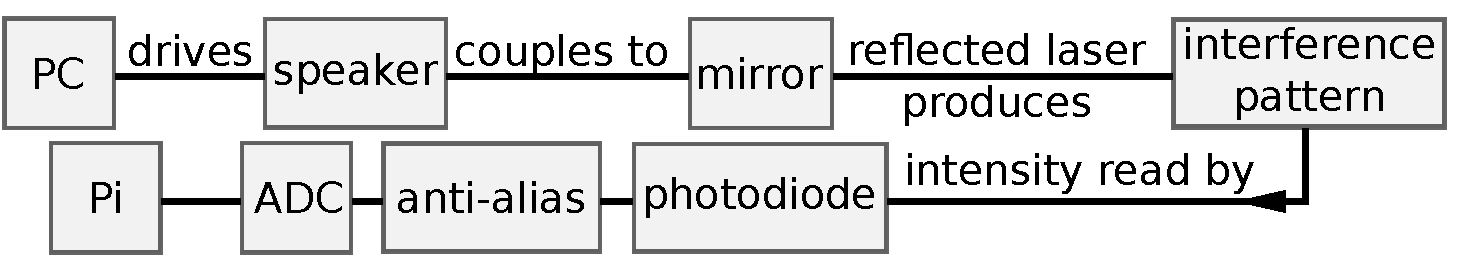
\includegraphics[width=.8\textwidth]{figures/pipeline_nobox.pdf}
	\caption{\label{fig:pipeline_highlighted}
Flowchart for the signal through the optical microphone. 
A transfer function of the system would have to account for each stage and exploration of this is an aim of future work. 
Not shown are the signal processing filters that are performed on the PC once the data is transferred off the Raspberry~Pi.
}
\end{figure*}

The experiment described here can be used to demonstrate and teach a variety of topics, from basic optics and photodiode circuits, to signal processing and speech enhancement. 
Cross-disciplinary undergraduate laboratory experiments between physics and engineering courses are beneficial to student learning (see Section II in the Supplementary Material for further information). 
% ``have been shown to be beneficial'' changed to ``are beneficial'' since we justify it elsewhere - james
Here, we consider further extensions and improvements to the experiment such as noise isolation, transfer function analysis, speech recognition, and control systems.



Isolating the experiment from interference may provide some noise reduction. 
The Raspberry Pi could be powered with a commercial battery instead of mains power, which may help to isolate the circuit from the mains as all other components draw power from the Raspberry~Pi (the laser is DC-powered through a converter).
Transferring the circuit from a breadboard to a printed circuit board can also reduce interference.\cite{elfekey2013design}
A feedback loop control system can also be used to suppress any unwanted movement of the interferometer components,\citep{abbott2017exploring, Sekiguchi:2016bmv, verhoeven2009robust} similar to methods used to isolate gravitational-wave observatories. 


A thorough characterization of the system's transfer function would allow us to understand how audio signals couple through the interferometer. 
The total transfer function starts with the voltage being sent to the speaker and ends with the voltage recorded by the Raspberry~Pi. 
It would include any inherent non-linearities in the speaker, the speaker-mirror coupling, the path length to intensity relation, and the photodiode. 
The schematic in Fig.~\ref{fig:pipeline_highlighted} shows the abstract signal flow through the system.
It does not include other potential pathways for signal flow such as acoustomechanical vibrations of the webcam or photodiode mount which could also be examined.


A voluminous literature exists on using hidden Markov models trained on phonemes to recognize speech.\cite{HMM_english}
These could perform the final stage of speech enhancement for the optical microphone. 
This coincidentally connects back to the Viterbi algorithm in Section~\ref{sec:viterbi_wandering}, which is also underpinned by a hidden Markov model, albeit of a different type. 
Alternatively, machine learning solutions exist throughout the field that can provide results competitive with statistical techniques (such as the logMMSE estimator used here).\cite{SEGAN}
%Alternatively, machine learning solutions exist throughout the field that can compete with statistical techniques such as the logMMSE estimator.\cite{SEGAN} \han{note}


More traditional techniques such as a wavelet transform~\citep{nason1995stationary} could be used to extract the signal from noise and compared with the above methods. 
A wavelet transform provides both time and frequency information, making it easier to pinpoint the origin of noise with respect to time. 
In Refs.~\cite{tufekci2000feature,agbinya1996discrete}, wavelet transform methods are proposed for speech recognition. 


Returning to the demonstration of gravitational wave analysis, single interferometers cannot yield directional information for signals; a large proportion of the directional information in gravitational-wave detections comes from the time delay offset between the signal\han{note} being recorded at two or more detectors.\cite{GW150914}
We could therefore extend this analysis to include data from two interferometers to extract directional information.
This would require increasing the sensitivity of the optical microphone to pick up the signal from a distant source instead of from a speaker attached directly to one of the mirrors of the interferometer.
Another extension would be to demonstrate the Doppler effect of the Earth's motion around the Sun, which needs to be considered in continuous-wave searches (see Section~\ref{sec:realCWSearches} and Ref.~\cite{JKS:1998}). 
One approach could be to modify the input audio signal to simulate Doppler modulation. 
% did we cut the turn-table idea? that was fun! - james
% yeah afraid so - it was nice, but the editor did not like it! :( - Hannah
% haha, okay. - james

\end{document}
